\section{Materials and Methods}

\subsection{Dataset, Split and Leakage Control}
We use only the TrialGPT Criterion Annotations file (1\,015 rows, 53 patients)~\cite{ncbi2024dataset}. Each row holds a patient note whose sentences are numbered (\texttt{0. \ldots}), a trial identifier and title, the criterion type and text, the expert label, and the expert evidence sentence IDs. The file also contains GPT-4 explanations, sentence IDs, labels and a correctness flag; these four columns are dropped at load time (\texttt{LEAKY\_COLUMNS} in \texttt{src/data.py}) so they cannot reach a prompt or a metric. The upstream \texttt{training} flag is ignored.

The split follows the assignment protocol: the 53 unique patient IDs are sorted, shuffled in place with \texttt{numpy.random.default\_rng(42)}, and the first 37, next 8 and last 8 IDs form train, validation and test. A programmatic check asserts that the three ID sets are disjoint, jointly cover all patients and account for every annotation; the manifest is saved as \texttt{data/processed/split\_manifest.json}. Table~\ref{tab:split} gives the resulting sizes. One annotation (ID 883) has no criterion text in the source file, so there is nothing to predict; it stays in the manifest counts but is excluded from training and evaluation, leaving \NTrain/\NVal/\NTest{} usable rows. Table~\ref{tab:labels} shows the label distribution: the classes \emph{excluded} and \emph{not included} are rare, and the test split contains no \emph{excluded} example at all, which affects how macro-F1 must be read.

\begin{table}[t]\centering\caption{Patient-grouped split (seed 42).}\label{tab:split}
\small\begin{tabular}{lrrrr}\toprule
Split & Patients & Annotations & Incl. & Excl. \\\midrule
train & 37 & 602 & 215 & 387 \\
validation & 8 & 206 & 66 & 140 \\
test & 8 & 206 & 75 & 131 \\
\bottomrule\end{tabular}
\end{table}
\begin{table}[t]\centering\caption{Expert label distribution per split (usable rows).}\label{tab:labels}
\small\begin{tabular}{lrrr}\toprule
Label & Train & Val. & Test \\\midrule
included & 88 & 35 & 27 \\
not included & 13 & 3 & 7 \\
excluded & 8 & 2 & 0 \\
not excluded & 291 & 101 & 91 \\
not enough info. & 174 & 53 & 66 \\
not applicable & 28 & 12 & 15 \\
\bottomrule\end{tabular}
\end{table}

\subsection{Task Formulation, Prompt and Output Schema}
The input is rendered through the model's ChatML template with a fixed system message, the numbered note, the criterion type, the criterion text and the list of labels allowed for that type (four per type: \emph{included/not included} or \emph{excluded/not excluded}, plus \emph{not enough information} and \emph{not applicable}). The target is a compact JSON object,
\begin{center}\small\texttt{\{"label": "not excluded", "evidence": [3, 5]\}}\end{center}
followed by the end-of-turn token. Evidence IDs are the original sentence IDs of the note, sorted ascending; an empty list is a legitimate answer. The parser accepts the JSON form, falls back to a lenient search for a label string, and marks anything else \emph{invalid}, which always counts as an error. Notes are short (mean prompt+answer length \TMeanTok{} tokens, maximum \TMaxTok{} with the SmolLM2 tokenizer), so with a 1\,024-token limit \textbf{no example is truncated} (\TTrunc{} truncations); the code nevertheless counts truncation events and would report them.

\subsection{Model Candidates and Selection}
We study two hardware tiers with the same model family. Table~\ref{tab:cand} lists the candidates with properties computed directly from each model's published \texttt{config.json}: parameter count, fp32 weight memory (parameters $\times$ 4 bytes), layers, query/key-value heads, vocabulary, context window, the fp32 KV-cache cost per token ($2\cdot L\cdot H_{kv}\cdot d_{head}\cdot 4$ bytes), and the role each model plays in this work. All four are Apache-2.0 licensed decoders (Llama-style for SmolLM2, Qwen2-style for Qwen2.5-0.5B). The figures are derived, not benchmarked; the training and inference times that actually decided the configuration are reported in Section~\ref{sec:results}.

\textbf{Configuration~A (GPU, headline).} Target \textbf{SmolLM2-1.7B-Instruct}: 1.71\,B parameters, 24 layers, hidden size 2\,048, 32 query heads with 32 key/value heads (multi-head attention, 64-dimensional heads), SwiGLU feed-forward of width 8\,192, rotary embeddings ($\theta=1.3\times10^5$), 8\,192-token context, tied embeddings, 49\,152-token vocabulary; about 6.85\,GB in fp32. It trains on a free 15\,GB T4 with LoRA and fp16 autocast. Draft \textbf{SmolLM2-360M-Instruct} (same tokenizer). Larger options (e.g.\ 7--8B models) would require 4-bit quantisation and CUDA-only libraries and were not considered.

\textbf{Configuration~B (CPU).} Target \textbf{SmolLM2-360M-Instruct}: 32 layers, hidden size 960, 15 query heads sharing 5 key/value heads (grouped-query attention), feed-forward width 2\,560, 8\,192-token context; about 1.45\,GB in fp32 and trainable in hours on four CPU cores. Draft \textbf{SmolLM2-135M-Instruct} (30 layers, hidden size 576, 9 heads / 3 KV heads), same 49\,152-token vocabulary. Qwen2.5-0.5B~\cite{qwen2024qwen25} (24 layers, hidden size 896, 14 heads / 2 KV heads, 151\,936-token vocabulary, 32\,768 context) was the alternative decoder: it has a three times larger embedding/softmax, query/key/value biases that our decoder would need to support, and no smaller member of its family to act as a same-tokenizer draft, so it was rejected (Table~\ref{tab:cand}).

\begin{table}[t]\centering\caption{Candidate decoders, computed from their configuration files (fp32 weights in decimal GB; KV = cache bytes per token in fp32).}\label{tab:cand}
\footnotesize\setlength{\tabcolsep}{2.5pt}\resizebox{\columnwidth}{!}{\begin{tabular}{lrrrrrrrl}\toprule
Model & Params & fp32 (GB) & Layers & Heads/KV & Vocab & Ctx & KV/token (kB) & Role \\\midrule
SmolLM2-1.7B & 1.71\,B & 6.85 & 24 & 32/32 & 49\,152 & 8\,192 & 393 & target (A) \\
SmolLM2-360M & 362\,M & 1.45 & 32 & 15/5 & 49\,152 & 8\,192 & 82 & target (B) / draft (A) \\
SmolLM2-135M & 135\,M & 0.54 & 30 & 9/3 & 49\,152 & 8\,192 & 46 & draft (B) \\
Qwen2.5-0.5B & 494\,M & 1.98 & 24 & 14/2 & 151\,936 & 32\,768 & 25 & rejected \\
\bottomrule\end{tabular}
}\end{table}

\subsection{Fine-Tuning}
LoRA adapters (rank $r=16$, $\alpha=32$, dropout 0.05) are attached to all seven linear projections of every layer (\texttt{q,k,v,o,gate,up,down}): 18.09M trainable parameters for the 1.7B target (1.05\%) and 8.68M for the 360M model (2.3\%). The objective is token-level cross-entropy computed \emph{only on the answer tokens} (the JSON string and end-of-turn token); prompt tokens are masked with $-100$, and the loss is normalised by the number of answer tokens in each optimizer batch. We use AdamW (weight decay 0.01), 10\% linear warm-up followed by cosine decay, gradient clipping at 1.0, effective batch size 16 via gradient accumulation, and seed 42. Configuration~A: learning rate $2\times10^{-4}$, 3 epochs for the 1.7B target (micro-batch 1), $3\times10^{-4}$ and 4 epochs for the 360M draft (micro-batch 4), fp16 autocast with a gradient scaler on a T4. Configuration~B: learning rate $3\times10^{-4}$, 2 epochs for the 360M target and 3 for the 135M draft, fp32 on CPU. After each epoch the script records validation loss and runs greedy generation on the validation split to obtain accuracy, macro-F1 and evidence F1; the adapter with the highest validation macro-F1 (ties broken by lower validation loss) is kept. The test split is never read by the training script. At inference the adapter is folded into the base weights as $W\leftarrow W+\tfrac{\alpha}{r}BA$ by our own loader (verified identical to the PEFT merge: maximum logit difference 0 on a test prompt), so no PEFT dependency is needed at serving time; the adapters are 72\,MB (1.7B), 35\,MB (360M) and about 13\,MB (135M).

\subsection{Explicit Decoder and KV Cache}
\label{sec:cache}
To control caching, masking and the attention kernel, we re-implemented the Llama forward pass (\texttt{src/minillama.py}) reading the Hugging Face safetensors. Correctness is checked against \texttt{LlamaForCausalLM} (Section~\ref{sec:kvres}). Fig.~\ref{fig:decoder}(a) shows one decoder step: new tokens are embedded, normalised and projected to queries, keys and values; rotary embeddings are applied with absolute positions; the rotated keys and values are written into the per-layer cache; the selected attention back-end reads the whole valid cache under the causal rule; and the usual output projection, residuals and SwiGLU feed-forward follow. Fig.~\ref{fig:decoder}(b) summarises the speculative round described in Section~\ref{sec:spec}.

\begin{figure*}[t]\centering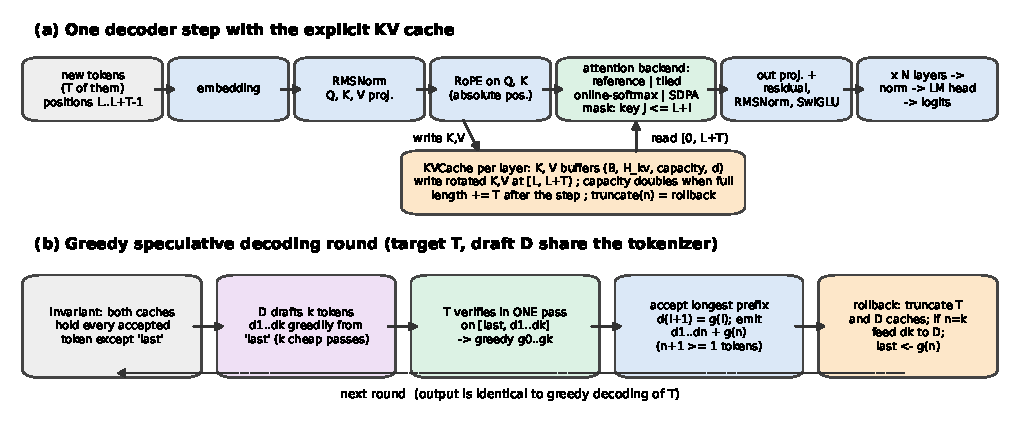
\includegraphics[width=.95\textwidth]{fig_decoder.pdf}
\caption{Architecture of our decoder implementation. (a) One forward step with the explicit, growable KV cache and the pluggable attention back-end (reference, tiled online-softmax, or PyTorch SDPA for comparison). (b) One round of greedy speculative decoding with cache rollback; the output equals greedy decoding of the target.}\label{fig:decoder}\end{figure*}

\emph{Positions.} Rotary embeddings rotate each query and key by its absolute position. For a step that feeds $T$ new tokens after $L$ cached ones, positions are $L,\dots,L+T-1$. Keys are rotated \emph{before} they are written to the cache, so cached keys already carry their position and are never rotated again; queries are rotated the same way and never cached.

\emph{Masking.} Query $i$ of the new block has absolute position $L+i$ and may attend to cache entry $j$ iff $j\le L+i$. During prefill ($L=0$) this is the usual lower-triangular mask; during one-token decoding ($T=1$) it admits the entire cache. The same \texttt{q\_offset} argument drives the mask in all attention back-ends.

\emph{Growth and rollback.} Each layer owns a pre-allocated key tensor and value tensor of shape $(B,H_{kv},C,d)$ with a shared length counter. New keys/values are written at slots $[L,L+T)$; if $L+T>C$ the capacity doubles (amortised $O(1)$ copies per token, in contrast to one \texttt{torch.cat} per step). Rolling back $n$ tokens is just setting the counter to $L-n$, which later writes overwrite---this is exactly what speculative decoding needs. With 32 layers, 5 KV heads and $d=64$, one cached token costs $2\cdot32\cdot5\cdot64\cdot4=82{,}000$ bytes in fp32 (about 80\,KB), i.e.\ 3$\times$ less than with 15 KV heads.

\emph{Numerical differences.} Cached and uncached paths compute the same mathematical function but with different matrix shapes (e.g.\ a $1\times d$ query against $L$ keys versus a full $T\times T$ product), which changes floating-point summation order. Logits can therefore differ at the $10^{-5}$ level, and a greedy argmax can flip only when the top-two logits are closer than that. We test token equality empirically (Section~\ref{sec:kvres}).

\subsection{Reference and Tiled Online-Softmax Attention}
\label{sec:attn}
The reference routine computes $S=QK^\top/\sqrt d$, applies the causal mask $M_{ij}=[j\le i+L]$ by setting masked scores to $-\infty$, subtracts the row maximum, exponentiates, normalises and multiplies by $V$; fully masked rows return zeros instead of NaN.

The tiled routine (Algorithm~\ref{alg:tiled}) never forms $S$. For each block of queries it sweeps over blocks of keys while keeping per-row statistics: the running maximum $m$, the running normaliser $\ell=\sum_j e^{s_j-m}$ and the running un-normalised output $o=\sum_j e^{s_j-m}v_j$. When a new key block with block maximum $\tilde m$ arrives, $m'=\max(m,\tilde m)$, the old statistics are rescaled by $\alpha=e^{m-m'}$, and the new block's contributions are added with the new maximum. The final output is $o/\ell$. Key blocks entirely above the causal diagonal are skipped, and grouped KV heads are broadcast to query heads block by block. PyTorch's fused \texttt{scaled\_dot\_product\_attention} is used only as a third comparison point.

\begin{algorithm}[t]\caption{Tiled attention with online softmax (one head)}\label{alg:tiled}
\begin{algorithmic}[1]
\small
\For{each query block $Q_b$ (rows $r$)}
 \State $m\gets-\infty,\ \ell\gets0,\ o\gets0$
 \For{each key block $K_c,V_c$ with $c$ not strictly above the diagonal}
  \State $S\gets Q_bK_c^\top/\sqrt d$; mask entries with key position $>$ query position
  \State $m'\gets\max(m,\mathrm{rowmax}(S))$;\ \ $\alpha\gets e^{m-m'}$;\ \ $P\gets e^{S-m'}$
  \State $\ell\gets\alpha\ell+\mathrm{rowsum}(P)$;\ \ $o\gets\alpha o+PV_c$;\ \ $m\gets m'$
 \EndFor
 \State output rows $\gets o/\ell$
\EndFor
\end{algorithmic}
\end{algorithm}

\subsection{Greedy Speculative Decoding}
\label{sec:spec}
Target (360M) and draft (135M) share the tokenizer, so token IDs are directly comparable. Both are held to one invariant at the start of each round: \emph{both caches contain every accepted token except the most recent one} ($\mathit{last}$). A round (Algorithm~\ref{alg:spec}) (1) lets the draft decode $k$ tokens from $\mathit{last}$, (2) runs \emph{one} target forward pass over $[\mathit{last},d_1,\dots,d_k]$, whose output at position $i$ is the target's greedy token $g_i$ after the $i$-th input, (3) accepts the longest prefix with $d_{i+1}=g_i$ and appends the target's own token $g_n$ (a correction at the first mismatch, or a free bonus token if all $k$ matched), and (4) restores the invariant: the target cache is truncated to keep only $\mathit{last},d_1..d_n$; the draft cache is truncated likewise, or, if all drafts were accepted, receives $d_k$ (which it had generated but never consumed). Each round therefore emits $n+1\ge1$ tokens and, by construction, the output equals greedy decoding of the target.

\begin{algorithm}[t]\caption{One round of greedy speculative decoding}\label{alg:spec}
\begin{algorithmic}[1]
\small
\State $d_1..d_k\gets$ draft greedy tokens starting from $\mathit{last}$ (draft cache grows by $k$)
\State $g_0..g_k\gets\arg\max$ of target logits on $[\mathit{last},d_1..d_k]$ (target cache grows by $k{+}1$)
\State $n\gets$ largest $n\le k$ with $d_i=g_{i-1}\ \forall i\le n$
\State emit $d_1..d_n,g_n$;\ \ target cache $\gets$ keep $\mathit{last},d_1..d_n$
\If{$n=k$} feed $d_k$ to the draft \Else{} truncate draft cache to $\mathit{last},d_1..d_n$ \EndIf
\State $\mathit{last}\gets g_n$
\end{algorithmic}
\end{algorithm}

\subsection{Criterion-Level Pipeline and Aggregation}
Fig.~\ref{fig:system} gives the end-to-end system: the offline training path (dataset, fixed split, prompt construction, LoRA fine-tuning, adapter selection) and the inference path used by the evaluation scripts and the browser application (input validation and sentence numbering, our decoder with the merged adapter under a chosen decoding mode, parsing, evidence extraction and explanation, rule-based aggregation, comparison view and report export).

\begin{figure*}[t]\centering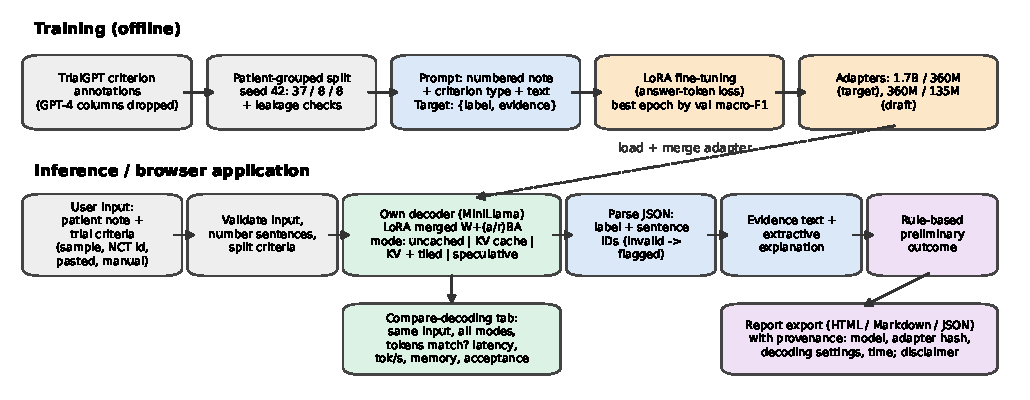
\includegraphics[width=.95\textwidth]{fig_system.pdf}
\caption{System architecture and application workflow. Top: offline training with the prescribed dataset and fixed split. Bottom: inference as used by evaluation and by the browser application.}\label{fig:system}\end{figure*}

For every criterion the pipeline returns: the criterion, predicted label, cited sentence IDs (IDs absent from the note are discarded and reported), the extracted text of those sentences, and an explanation. The explanation is a deterministic template that restates the label and quotes only the cited sentences; for \emph{not enough information} it states that missing mention is not evidence either way. We deliberately do not train on or generate free-text rationales, because the only rationales in the corpus are GPT-4 outputs that the protocol forbids. A patient--trial \emph{preliminary outcome} is an explicit rule over the criterion labels, not a learned or ground-truth label: any inclusion \emph{not included} or exclusion \emph{excluded} gives ``likely not eligible''; otherwise any \emph{not enough information} or invalid output gives ``needs more information''; otherwise ``potentially eligible''.

\subsection{Application}
\label{sec:app}
The application (FastAPI back-end, single-page browser UI, \texttt{app/}) loads the target and draft once, then lets a user paste a note (auto-numbered when needed), choose a held-out sample trial, fetch one from ClinicalTrials.gov by NCT ID (metadata only), or paste an eligibility block that is split into criteria. It shows each criterion's label, cited sentences highlighted in the numbered note, the explanation and raw output, and a rule-based overall outcome; reports are exported as HTML, Markdown or JSON with model, adapter hash, decoding settings and time stamp. A \emph{Compare decoding} tab runs the current input through all four decoding modes on the user's machine and tabulates tokens-match, latency, throughput, memory and acceptance rate; an \emph{Experiments} tab renders the stored result files. Invalid input (short notes, unknown criterion types, empty reports, unreachable trial registry) is rejected with explanatory messages. A banner states that this is an educational screening prototype and not a clinical enrollment decision.
